\mysubsectionformatted{Design Pattern Do It Myself}
\myparagraph{
    \begin{tcolorbox}[colback=blue!5!white, colframe=blue!75!black]
        Chiamato così da Peter Coad, il pattern ha l'obiettivo di applicare il \textbf{Polimorfismo},
        quindi far si che un oggetto software faccia quelle operazioni che normalmente
        verrebbero fatte all'oggetto reale di cui loro sono un'astrazione (loro intesi come gli oggetti software).  
    \end{tcolorbox}

    Detto in modo informale:
    \begin{itemize}
        \item Gli oggetti Quadrato creano se stessi.
        \item Gli oggetti Cerchio creano se stessi.
        \item Gli oggetti Text eseguono il controllo ortografico di se stessi.
    \end{itemize}

    \setcounter{figure}{0}
    \begin{figure}[h]
        \centering
        \caption{Uso del Polimorfismo con i mezzi di pagamento}
        \vspace{0.5cm}
        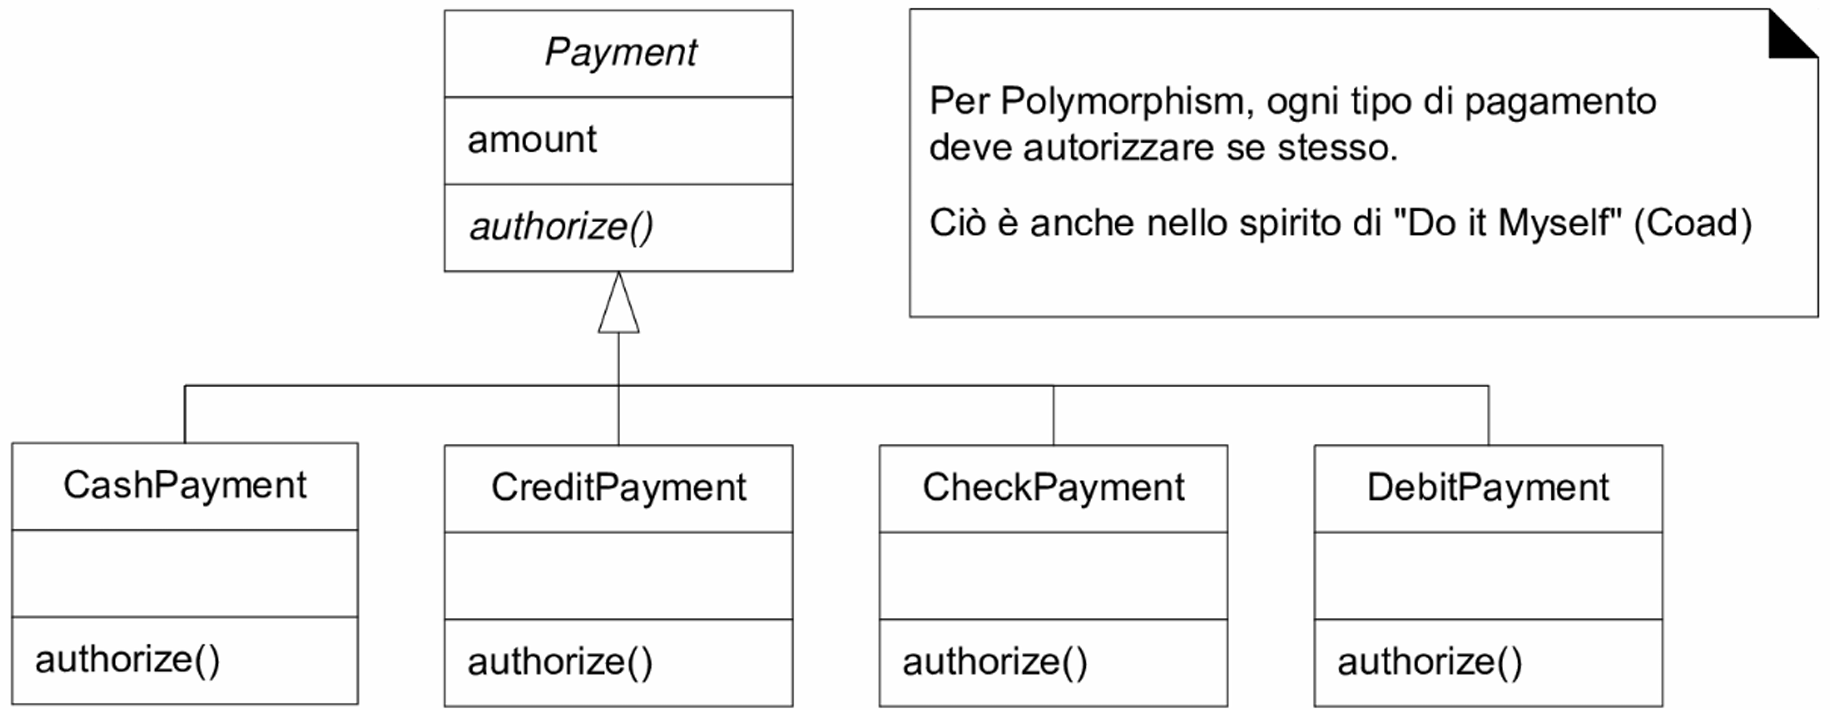
\includegraphics[scale=0.25]{Esercitazione - Design Patterns/Polymorphism.png}
        \label{fig:polymorphism}
    \end{figure}
}
\newpage